\section{Domain Name System}

Mapea direcciones (IP/IPv6) a nombres. Los nombres se pueden jerarquizar de dos formas: organizacionalmente y territorialmente. Funciona sobre UDP y utiliza TCP para transferencia de zonas, ambas en puerto 53.

\begin{figure}[H]
    \centering
    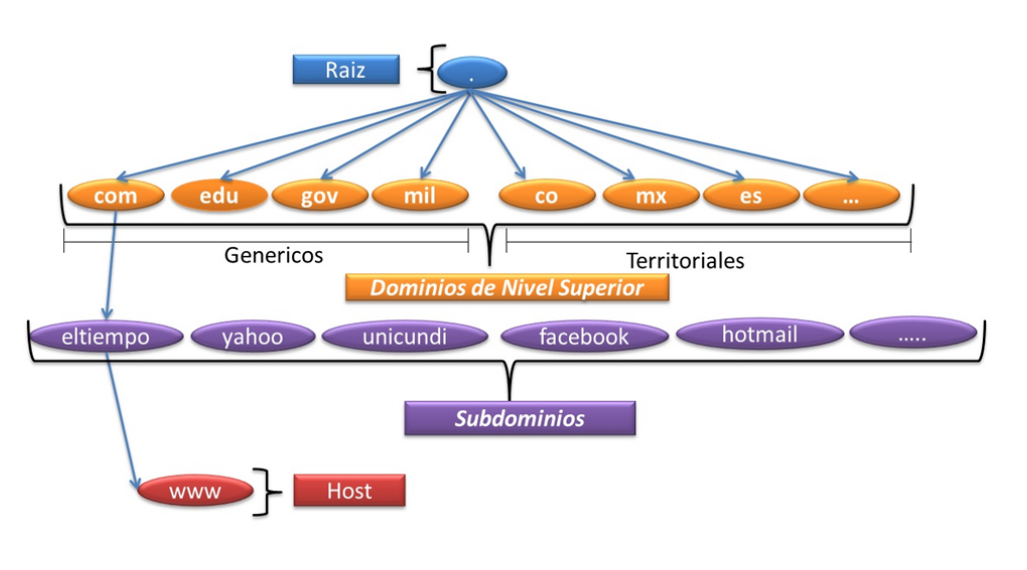
\includegraphics[width=0.5\textwidth]{capitulos/dns/imagenes/jerarquia.png}
    \caption{Jerarquía de nombres DNS}
    \label{fig:dns-jerarquia}
\end{figure}

\begin{definicion}{Zonas}
    Llamamos zona a la undad de administración delegada a un individuo o organización. Es la administración de un determinado espacio de nombres DNS.
\end{definicion}

\begin{figure}[H]
    \centering
    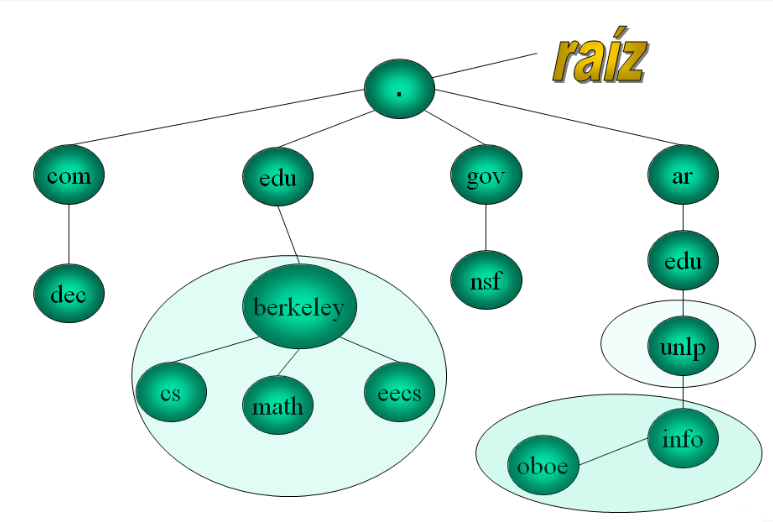
\includegraphics[width=0.5\textwidth]{capitulos/dns/imagenes/zonas.png}
    \caption{Visualización de zonas DNS}
    \label{fig:dns-zonas}
\end{figure}


\subsection{Registros de Recursos}

Son los nombres lógicos con los que se almacenan los datos del servidor.

\begin{itemize}[label=\textcolor{acento}{$\bullet$}]
    \item \textbf{A (Address):} mapea un nombre a una dirección IP.
    \item \textbf{PTR (Pointer):} mapea una dirección IP a un nombre (vice-versa de A).
    \item \textbf{CNAME (Canonical Name):} apunta a otro nombre, se lo conoce como \emph{alias}.
    \item \textbf{MX (Mail Exchanger):} registro que hace funcionar al correo electrónico. Le dice a todo Internet \textbf{qué servidor es el encargado de recibir los mails} de ese dominio.
    \item \textbf{NS (Name Server):} indica cuáles son los servidores DNS que tienen la información oficial y actualizada.
    \item \textbf{SOA (Start Of Authority):} para pedir parámetros del dominio.
\end{itemize}

\subsection{Servidores DNS}

El \textbf{servidor raíz} delega a todos TLDs, y no permite consultas recursivas. Proporcionan referencias directas a servidores dedominio de segundo nivel (com, edu, gov, ...). Los \textbf{servidores autoritativos} se encargan de una zona o sub-dominio de nombres, y puede subdelegar.

Los \textbf{servidores locales} son los que se consultan dentro de una red. Mantienen caché, permiten consultas recursivas a los hosts internos y pueden ser autoritativos. 

Luego están los \textbf{Open Name Servers}, que son servidores de DNS que funcioan como si fueran locales para cualquier cliente. Los \textbf{Forwarded Name Servers} funcionan como proxies de otros DNSs internos, e interactúan directamente con el sistema DNS exterior.

Los \textbf{Primary Name Servers} almacenan la información de su zona en una database local, y son responsables de mantener la información actualizada. Los \textbf{Secondary Name Servers} obtienen los datos desde otro servidor que tenga la autoridad para esa zona, y copia la información. Este proceso se llama \emph{transferencia de zona} y en vez de hacerse por UDP se hace por TCP.

\subsection{Proceso de Consulta}

\begin{tcolorbox}[
    enhanced,
    colback=green!2!white,        % Fondo verde muy suave
    colframe=green!50!black,      % Borde verde oscuro elegante
    title=\textbf{Mecanismo de Resolución de Nombres (DNS)},
    fonttitle=\large\sffamily,    % Fuente del título sin serifas
    coltitle=white,
    boxrule=1.2pt,
    arc=6pt,                      % Bordes redondeados
    drop shadow=black!15!white,   % Sombra sutil
    left=10pt, right=10pt, top=10pt, bottom=10pt
]

Todo host cuenta con la configuración de un \textbf{servidor DNS local} (resolver). Cuando un dispositivo necesita resolver un nombre de dominio, envía su petición inicial a este servidor local, a partir de lo cual pueden darse dos escenarios:

\begin{itemize}[leftmargin=*, label=\textcolor{green!50!black}{\textbullet}]
    \item \textbf{Respuesta Autoritativa (Fidedigna):} Si el servidor local es la autoridad para el dominio consultado, significa que aloja exactamente esa porción de la base de datos distribuida. En este caso, posee el mapeo directo y le devuelve la respuesta al host de forma inmediata.
    
    \item \textbf{Búsqueda Externa (Delegación):} Si el servidor local no es fidedigno para dicho dominio, deberá iniciar una búsqueda externa consultando a un \textbf{Root Server} (Servidor Raíz).
\end{itemize}

\vspace{0.2cm}
\noindent\textbf{Dinámica de Peticiones (Recursivas vs. Iterativas):} \\
Para evitar la sobrecarga y el colapso de la infraestructura global, la petición dirigida al Root Server es estrictamente \textbf{iterativa}. El Root Server no busca la IP final, sino que se limita a devolver la dirección de un servidor intermedio (como un servidor TLD). 

A partir de allí, el servidor local envía una petición \textbf{recursiva} a este servidor intermedio. Al ser recursiva, le delega la responsabilidad de continuar interrogando a la jerarquía de servidores hasta alcanzar al servidor fidedigno definitivo. Una vez hallado el mapeo correcto, la respuesta viaja de regreso hasta llegar al host original.

\end{tcolorbox}

Se utiliza \textbf{Caching} para reducir el tráfico en búsquedas de dominios no locales, donde las entradas a esta memoria se temporizan.  

\subsection{Flags DNS}

Cuando realizamos una \textbf{consulta DNS}, la misma puede retornar distintos flags.

\begin{itemize}[leftmargin=*, label=\textcolor{acento}{$\bullet$}]
    \item \textbf{qr:} query.
    \item \textbf{rd:} recursion desired, el cliente desea que la consulta se resuelva recursivamente.
    \item \textbf{ra:} recursion available, el servidor tiene la recursión habilitada.
\end{itemize}

El \textbf{TTL} (Time to Live) indica el tiempo que se mantiene la respuesta en caché (en segundos).

